Timing noise refers to small, low level structure in the timing residual which
cannot be attributed to any other source, an example is given in figure
\ref{fig: timing noise example}. The amount of timing noise will depend on the
order of truncation of the Taylor expansion.  In most studies, and so in this
work, we will truncate at $n=3$, the second order spindown; the timing noise is
then the residual left after a $n=3$ fit. Increasing this truncation level can
fit out these variations, but we are interested in understanding the origins
and implications of timing noise.

\begin{figure}[htb] 
    \centering
    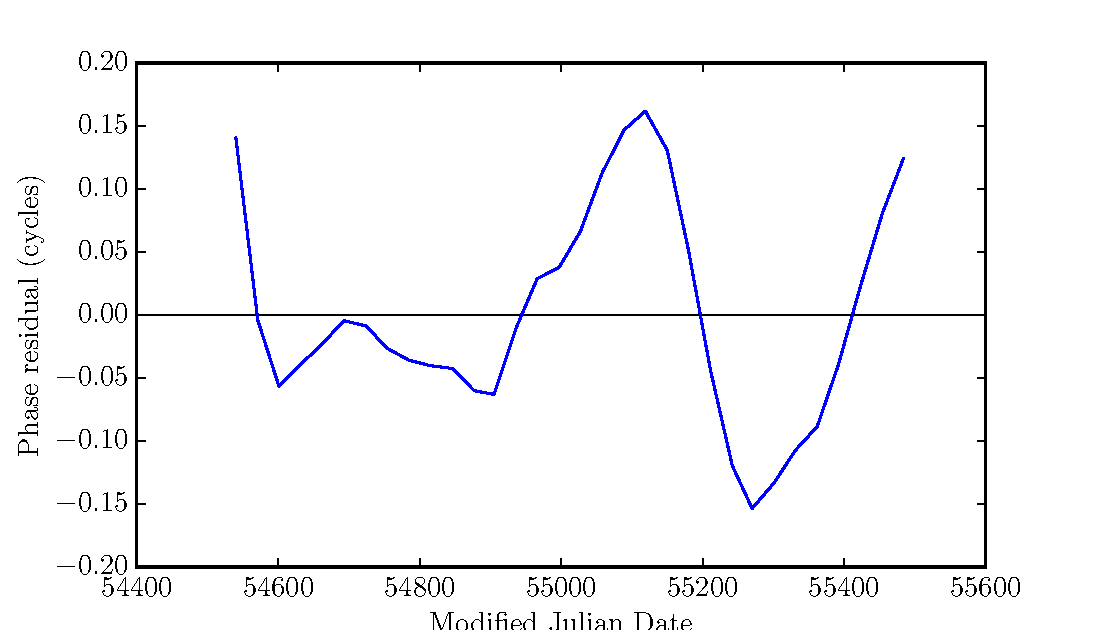
\includegraphics[width=0.75\textwidth]{Crab_residual_phase}
    \caption{A timing residual demonstrating structure which is named timing
        noise.  This is generated from data on the Crab ephemeris (see section
    \ref{sec: timing noise as described by the crab ephemeris})}
    \label{fig: timing noise example}
\end{figure} 

There have been various attempts to characterise timing noise
over the history of 
pulsar astronomy. Most observations are tied to a particular interpretation
which we will discuss in part \ref{sec: interpretations of timing noise}.
It is however worth first listing some of the model independent observations.
These are summarised by the most comprehensive study of timing noise from 
\citet{Hobbs2010} who considered 366 pulsars over time scales $\gtrsim10$~years.
They found that:
\begin{enumerate}

    \item Timing noise is widespread in pulsars

    \item Timing noise is inversely correlated the characteristic age
        defined in equation \ref{eqn: characteristic age}

    \item The structures seen in the timing residual vary with data span. As
        more data is collected, more quasi-periodic features are observed.

    \item The dominant contribution to timing noise for young pulsars with
        $\tau_{c}<10^{5}$~years can be explained as being caused by the
        recovery from previous glitches.

    \item A handful of pulsars exhibit significant periodicity's while
        quasi-periodicity's are observed in many pulsars

\end{enumerate}


